\chapter{Results}
\section{Overview}
Tests were conducted between the 1st of April and the 11th 2025. The OONI probe App was also ran on occasion on Windows and mobile devices, though this test suite is far less comprehensive in comparison to the CLI. 

It is important to recognize that, particularly in the case of Israel, different individuals may experience censorship of the Internet to varying degrees. The research focuses on replicating the experience of the average Israeli living in Tel Aviv. Having previously discussed the Gaza Strip, it is clear that the user experience varies greatly between the two areas. Further research may look at comparing Internet censorship experienced internally in Israel, but that is outside the scope of this work.

In the following section, the relevant context regarding the network conditions while gathering ground truth will be discussed. Having previously highlighted the varying levels at which internet censorship can be conducted, let us now define the specific network characteristics under which the OONI probe was run for both countries.

\subsection{Network Environment Context: Ireland}
As mentioned, the OONI CLI probe is running on a Raspberry Pi 5 connected to a home residential network over WiFi. The provider is Virgin Media (AS12388), registered under Liberty Global B.V. ISP (AS6830). 

Details regarding the operating system flashed to the Raspberry Pi and packages required for this are illustrated below in the 'Guide to Replicating Results.' 

\subsection{Network Environment Context: Israel}
Ground truth gathering in Israel was done using a virtual machine as described in the section on methodology. The virtual machine is operates within a data center hosted by O.M.C. COMPUTERS \& COMMUNICATIONS LTD (AS44709), downstream of its owner Kamatera Inc. (AS36007). This differs from the residential network that is being tested in Ireland.


\section{Website Connectivity Tests}
\subsection{Public OONI Database}
\subsection{Ground Truth via SSH}


\section{Circumvention Tests}
\subsection{Public OONI Database}
\subsection{Ground Truth via SSH}

\section{Instant Messaging Tests}
\subsection{Public OONI Database}
\subsection{Ground Truth via SSH}

\section{Middlebox Tests}
\subsection{Public OONI Database}
\subsection{Ground Truth via SSH}

\section{Comparitive Analysis: Ireland vs. Israel}
\subsection{Summary: Irish Internet Censorship}
\subsection{Summary: Israeli Internet Censorship}
\subsection{}

\section{Guide to Replicating Results}

\subsection{Raspberry Pi Setup}
\textbf{Operating System}
The operating system used was the latest available version of Raspberry Pi OS (64-bit) at the time of testing. It was flashed using the Raspberry Pi Imager application over USB. 

\begin{flushleft}
\hspace{1em}\textbf{Raspberry Pi OS (64-bit)}\\[0.5em]
\hspace{1em}Release date: November 19th 2024\\[0.5em]
\hspace{1em}System: 64-bit\\[0.5em]
\hspace{1em}Kernel version: 6.6\\[0.5em]
\hspace{1em}Debian version: 12 (bookworm)
\end{flushleft}


\textbf{Packages Installed}
In order to install the OONI probe CLI, the guide 'Install OONI Probe CLI on Debian/Ubuntu Linux' \cite{ooni-cli-install}. The process was similar to that of installing on the Israeli VM. One obstacle faced in both instances were OpenPGP errors. To solve, the permissions for OONI probe had to be updated to bypass PGP signature verification. To do this, /etc/apt/sources.list.d/ooniprobe.list was edited to include '[trusted=yes]'
\begin{figure}
    \centering
    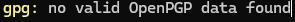
\includegraphics[width=0.5\linewidth]{PGPERROR.png}
    \caption{PGP Error installing CLI}
    \label{fig:enter-label}
\end{figure}


\begin{table}
\centering
\caption{Summary of Blocked vs. Unblocked Websites by Country}
\begin{tabular}{lcc}
\toprule
\textbf{Country} & \textbf{Unblocked} & \textbf{Blocked} \\
\midrule
Ireland & XXX & XXX \\
Israel    & XXX & XXX \\   
\bottomrule
\end{tabular}
\label{tab:blocked_summary}
\end{table}